\chapter{UMAP}

    \section{Fondements et intuition}
        \textit{
        Expliquer ce que tu vas traiter (catégories non)
        \\
        Intuition sur la théorie des catégories et géo diff
        \\
        Présentation des 4 grands hyperamètres
        }
        \\
        \\
        On souhaiterait être à nouveau capable de choisir la dimension de réduction, et projeter de manière intelligente les données dans cet espace en mettant l’accent sur des structures locale des données.
        \\
        \\
        Leland McInnes, John Healy et James Melville publient en 2018 l’article UMAP : Uniform manifold approximation and projection for dimension reduction. L’algorithme présenté est UMAP et répond à ce souhait. La théorie des catégories et des notions de la géométrie différentielles sont exploités pour donner un cadre mathématiques de très grande qualité à cette algorithme. Nous ne recommandons donc pas de lire en détail la partie théorique de l’article, et nous n’allons que donner les intuitions et problèmes qui sont discuté dans cette partie-là.
        \\
        \\
        L’idée de l’algorithme est de fonctionner en deux temps. Dans un premier temps on apprend la structure des données (locale) dans l’espace de départ, puis on essaye de trouver le meilleur moyen possible pour projeter de l’espace de départ à celui de réduction. Avant de traiter en détails ces deux parties, laissons-nous guider par les hyper-paramètres de cet algorithme :
        \begin{itemize}
            \item n : nombre de voisin à considérer dans l’espace de départ pour apprendre la structure des données
            \item d : la dimension de l’ensemble de réduction
            \item min\_dist : la séparation souhaité entre deux points proche dans l’espace de réduction
            \item n\_epochs : le nombre d’itération d’optimisation pour la projection dans l’espace de réduction
        \end{itemize}
        Avec cela, nous comprenons que choisissons vraiment la dimension de l’espace d’arrivé ! C’est un point fort par rapport à Johnson-Lindenstrauss où nous avons une borne et des conditions supplémentaires, et par rapport à l’analyse par composante principale où l’on sélectionne les composantes en essayant d’avoir une explication de la variance suffisamment forte.
        \\
        \\
        Egalement, il semblerait que le placement des points dans l’espace de réduction soit itératif, donc il y aurait un problème d’optimisation à résoudre. Il nous reste à comprendre le fonctionnement des deux étapes de l’algorithme pour comprendre l’utilité des deux hyper-paramètres restant.








    \section{Générer le graphe en grande dimension}
        \textit{
        Comment on s'en sort du fléau ?
        \\
        Quels difficultés mathématiques ?
        \\
        Hadamard / t-norm/conorm
        }
        \\
        \\
        Pour un point donné, on cherche à trouver son voisinage pour estimer sa densité. Cependant, puisque nous sommes potentiellement en grande dimension, nous aurons des problèmes liés au fléau de la dimension. Pour s’en sortir on décide de munir chaque point d’un espace avec sa propre métrique. On s’assure de revenir dans un espace de dimension bien plus petit et également d’avoir une notion de distance cohérente (puisqu’on peut normaliser la distance par rapport au voisin le plus éloigné). Ainsi, nous pouvons prendre des boules de rayon 1 pour chaque point avec sa propre distance et en réalité s’assurer que chaque point possède bien k voisins à l’intérieur de sa boule.
        \\
        \\
        En faisant cela, on résout des problèmes mais on en crée un de taille : nous n’avons plus de cohérence globale. Ainsi, la partie la plus mathématiques de cet article adresse cette problématique et défini un nouveau type d’objet qui permet de définir une structure cohérente à plus haut niveau, en contre partie de la perte de certitude sur l’appartenance ou non de point à un voisinage donné. C’est le choix de travailler avec un nombre de voisin variable qui nous permet de simplifier l’écriture de cette partie plutôt que d’avoir des rayons variables.
        \\
        \\
        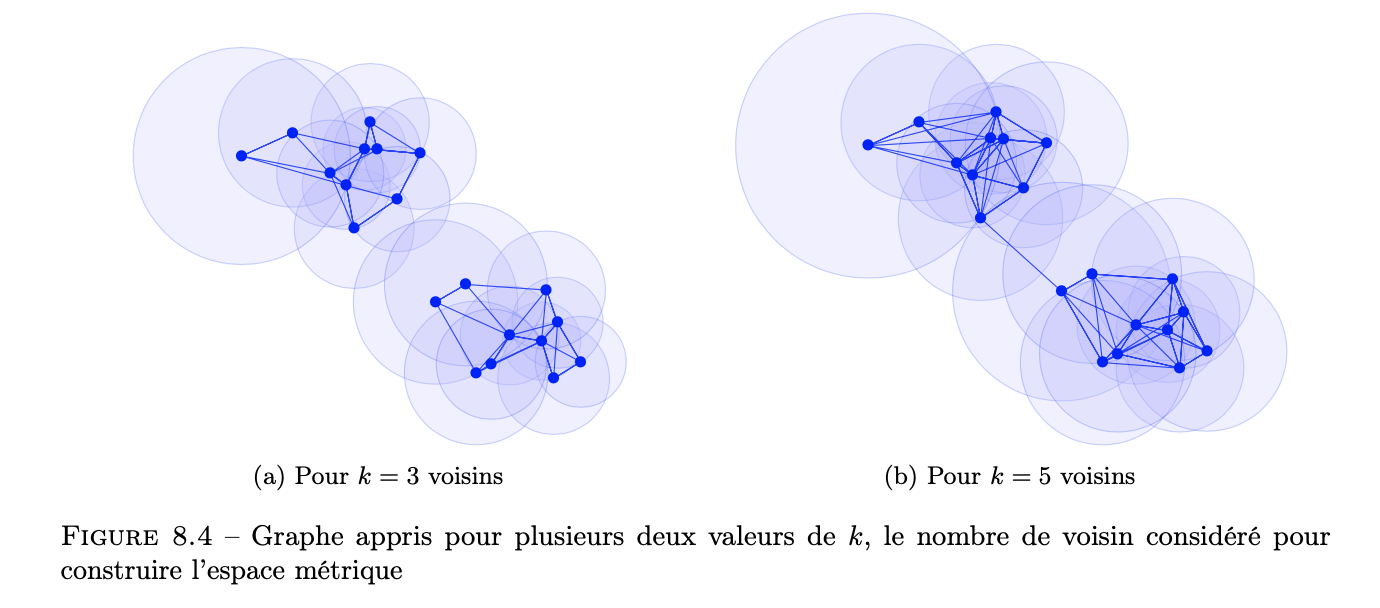
\includegraphics[width=\linewidth]{./img/umap/graph}
        \\
        \\
        Toutes ces intuitions mathématiques se réalisent concrètement sous la forme d’un graphe dirigé où chaque arrête possède un point. Plus formellement, pour chaque point $x_i$, on commence par trouver ses k voisins les plus proches selon la distance $d$ que l’on aura sélectionné. On note cette ensemble $\mathcal{N} (xi) = {x(1), . . . x(k)}$. On peut donc définir :
        \\
        \begin{eqnarray}
            \rho_i = min\{d(x_i, x_i^{(j)})|1 \leqslant j \leqslant k, d(x_i, x_i^{(j)}) > 0 \}
        \end{eqnarray}
        \\
        Cette définition de $\rho_i$ dérive de contrainte théorique : il s’agit de s’assurer que $xi$ sera connecté à au moins un autre point du dataset que l’on considère avec un poids d’arrête qui vaut 1.
        \\
        Puis on définit un coefficient de normalisation $\sigma_i$ qui est solution de l’équation :
        \\
        \\
        
\includegraphics[width=\linewidth]{./img/umap/eq_1}
        \\
        \\
        Ce coefficient permet de normaliser les distances locale pour chaque point $xi$. Tout cela nous permet de définir le poids d’une arrête comme :   
        \\
        \\
        
\includegraphics[width=\linewidth]{./img/umap/eq_2}
        \\
        \\
        Nous avons maintenant réussi à construire un graphe orienté à partir des données d’entrée, et l’on note $A$ la matrice adjacente au graphe $\overline{\rm G}$. On peut interpréter chaque coefficient $A_{ij}$ de $A$ comme la probabilité que l’arrête de $x_i$ vers $x_j$ existe.
        Si l’on considère maintenant la matrice $B$ définie par :
        \\
        \begin{eqnarray}
            B = A + A^t - A \circ A^t
        \end{eqnarray}
        \\
        Avec $\circ$ la notation du produit Hadamard définit par $(U \circ V)_{ij} = U_{ij}V_{ij}$. Autrement dit : il s’agit du produit terme à terme de deux matrices de même tailles.
        \\
        \\
        Soient $U, V \in \mathcal{M}_{n,m}$. On rappelle que : 
            $(U+V)^t = U^t + V^t$
            $(U \circ V)^t = U^t \circ V^t$
        \\
        \\
        \textbf{Montrer que la matrice B est symétrique : }
        \\
        \\
        On a :
        \\
        \begin{eqnarray}
            B^t  = (A + A^t - A \circ A^t)^t 
                = A^t + A - A^t \circ A
                = A + A^t - A \circ A^t
        \end{eqnarray}
        \\
        Ainsi, $B = B^t$ donc $B$ est symétrique.
        \\
        Alors on peut interpréter chaque coefficient $B_{ij}$ comme la probabilité que au moins une des deux
        arrêtes existe ($x_i$ vers $x_j$ ou $x_j$ vers $x_i$).
        Ainsi on définit le graphe UMAP $G$ avec la matrice adjacente donnée par $B$. Il nous reste maintenant
        à le réduire.



        \subsection*{Fuzzy Logical}







    \section{Réduction du graphe en petite dimension}
        \textit{
        \\
        Spectral embedding
        \\
        Problème force directed layout
        }
        \\
        \\
        UMAP utilise un algorithme force-based layout ou algorithme de dessin basé sur des forces en français. Ce fonctionnement exploite des forces attractives et répulsive sur les arcs et les noeuds. L’idée est de resserrer les liens et d’éloigner les observations.
        \\
        \\
        La force attractive entre deux noeuds xi et xj de coordonnées respective yi et yj est donnée par :
        \\
        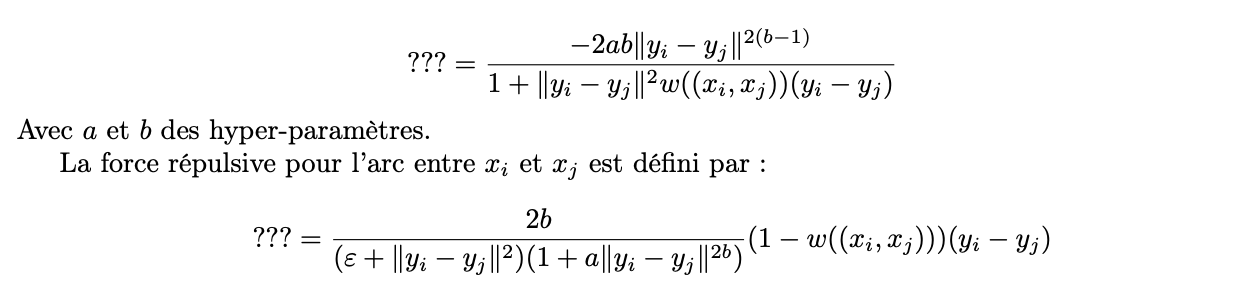
\includegraphics[width=\linewidth]{./img/umap/reduction_dim}
        \\
        \\
        L'algorithme peut être initialisé aléatoirement mais en pratique, puisque le Laplacien symétrique du graphe G est une approximation discrète de l'opérateur de Laplace-Beltrami du manifold, nous pouvons utiliser une incorporation spectrale (Spectral embedding) pour initialiser la réduction. Cette méthode permet à la fois une convergence plus rapide et une plus grande stabilité au sein de l'algorithme.




        \subsection*{Spectral embedding}
        L'incorporation spectrale est une technique utilisée pour la réduction non linéaire de la dimension. Il s'agit de l'algorithme des valeurs propres de Laplace, son objectif est de préserver la géométrie locale, c'est-à-dire que les points proches dans l'espace original restent proches dans l'espace réduit.
        \\
        \\
        Cette technique repose sur l'hypothèse de base selon laquelle les données se trouvent dans un manifold de faible dimension dans un espace de haute dimension. 
        \\
        \\
        L'algorithme d'incorporation spectrale se décompose en trois étapes :
        \begin{enumerate}
            \item Construction du graph adjacent
            \item Choisir les poids
            \item Obtention des valeur propres
        \end{enumerate}

            \subsubsection*{Construction du graphe d'adjacent}
            La première étape consiste à construire un graphe d'adjacence basé sur les données données. Nous plaçons une arête entre les nœuds i et j si les points de données correspondants sont "proches" : 
            \begin{itemize}
                \item \textbf{Nearest Neighbors :} Deux points, $x_i$ et $x_j$ sont reliés par une arête si l'un fait partie des K plus proches voisins de l'autre.
            \end{itemize}


            \subsubsection*{Choisir les poids}
            Maintenant, l'étape suivante consiste à pondérer les bords que nous avons définis dans la première étape. Ici, nous avons deux variantes différentes :
            \begin{itemize}
                \item \textbf{Pondération Gaussienne :} Si les nœuds i et j ne sont pas connectés alors mettez $W_{ij}$ = 0, sinon utilisez la formulation, $W_{ij} = exp[-||x_i - x_j|^2/ t]$.
                \item \textbf{0/1 Pondérations :} $W_{ij}$ = 1 si les sommets i et j sont reliés par une arête, sinon mettre $W_{ij} = 0$.
            \end{itemize}



            \subsubsection*{Obtention des valeur propres}
            Après la deuxième étape, nous aurons la matrice de poids $(W)$ avec nous. En utilisant W, nous obtiendrons la matrice de poids diagonale $(D)$, dont les entrées sont des sommes de colonnes (ou de lignes, puisque W est symétrique) de W, c'est-à-dire $D_{ii} = \Sigma_i W_{ij}$. Une fois que nous avons obtenu D, nous allons obtenir la matrice laplacienne $(L)$, où $L = D-W$.










    \section{UMAP : utilisation}
        \subsection{En pratique}
        hyperparamètres supplémentaires...

        \subsection{Test puis exploitation}
        Explications